\documentclass[12pt,a4paper,twoside]{article}
\usepackage{definitions}

\setlength{\voffset}{-28.4mm}
\setlength{\hoffset}{-1in}
\setlength{\topmargin}{20mm}
\setlength{\oddsidemargin}{25mm}
\setlength{\evensidemargin}{25mm}
\setlength{\textwidth}{160mm}

\setlength{\parindent}{0pt}

\setlength{\textheight}{235mm}
\setlength{\footskip}{20mm}
\setlength{\headsep}{50pt}
\setlength{\headheight}{0pt}

\begin{document}
\pagestyle{empty}
%%%% Title page
\begin{titlepage}
\begin{center}

\includegraphics{TUMlschwarz.png}\\[3mm]
\sf
{\Large
  Technische Universit\"at M\"unchen\\[5mm]
  Department of Mathematics\\[8mm]
}
\normalsize
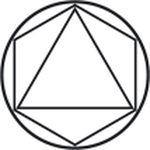
\includegraphics{TUMlMschwarz.png}\\[15mm]

Master's Thesis\\[15mm]

{\Huge
  Title
}
\bigskip

\normalsize

Florian Rohm
\end{center}
\vspace*{75mm}

Supervisor: Prof.\ Dr.\ Barbara Wohlmuth

\medskip

Advisor: M.Sc. Ehsan Fattahi Evati
\medskip

Submission Date: \ldots

\end{titlepage}
%%%% The following has to be signed by hand!

\vspace*{150mm}

I assure the single handed composition of this master's thesis only supported by declared resources.
\bigskip

Garching,
\newpage
%%%% Zusammenfassung in deutscher Sprache
\section*{Zusammenfassung}
Bei einer in englischer Sprache verfassten Arbeit muss eine Zusammenfassung in deutscher Sprache vorangestellt werden.
Daf\"ur ist hier Platz.

\newpage
\tableofcontents
\newpage

%%%% Page numbering restarts here
\pagenumbering{arabic}
\pagestyle{headings}

%%%%%%%%%%
\section{History of Lattice Boltzmann}
\label{sec:History of Lattice Boltzmann}
\cite{geier2015cumulant}
\cite[Page 1]{d1994generalized}
\cite{harris2004introduction}
Tell a bit about the two views of lbm, historically from Lattice Gas, see nowadays as numerical scheme for discrete boltzmann equation

%%%%%%%%%%
\section{Lattice Boltzman basics}
\label{sec:Lattice Boltzman basics}

\subsection{Stream and Collide}
\label{sub:Stream and Collide}

\subsection{Moments and physical quantities}
\label{sub:Moments and physical quantities}

\subsection{The issue with relaxation rates}
\label{sub:The issue with relaxation rates}
A bit about how fast we go to local equilibrium, coupling of independent processes

\subsection{Cumulants}
\label{sub:Cumulants}
What are cumulants, why are they a good choice

%%%%%%%%%%
\section{Transformations}
\label{sec:Transformations}

\subsection{Cumulants from moments}
\label{sub:Cumulants from moments}

\subsection{Central moments from cumulants}
\label{sub:Central moments from cumulants}

\subsection{Cumulants from central moments}
\label{sub:Cumulants from central moments}

\subsection{Fast central moment transformation}
\label{sub:Fast central moment transformation}

%%%%%%%%%%
\section{The cumulant collision}
\label{sec:The cumulant collision}

\subsection{The Maxwell-distribution}
\label{sub:The Maxwell-distribution}

\subsection{Equilibrium distribution for cumulants}
\label{sub:Equilibrium distribution for cumulants}

\subsection{Equilibrium in terms of moments}
\label{sub:Equilibrium in terms of moments}

\subsection{Choosing the \texorpdfstring{$\omega_i$}{omega i}}
\label{sub:Choosing the omega i}

%%%%%%%%%%
\section{Series expansions}
\label{sec:Series expansions}
After presenting the method, we need to proove that it satisfies Navier-Stokes.
Preparation

\subsection{Expanding the Lattice Boltzmann equation}
\label{sub:Expanding the Lattice Boltzmann equation}

\subsection{Matching the coefficients}
\label{sub:Matching the coefficients}

\subsection{Expanding the normalized cumulants}
\label{sub:Expanding the normalized cumulants}

\subsection{Expanding the equilibrium moments}
\label{sub:Expanding the equilibrium moments}

\subsection{Collision of moments}
\label{sub:Collision of moments}

%%%%%%%%%%
\section{Continuity equation}
\label{sec:Continuity equation}

\subsection{Assumptions}
\label{sub:Assumptions}

\subsubsection{Absence of sources}
\label{subs:Absence of sources}

\subsubsection{Derivatives of zeroth order terms}
\label{subs:Derivatives of zeroth order terms}

\subsection{Collision invariants}
\label{sub:Collision invariants}

\subsection{Deriving the continuity equation}
\label{sub:Deriving the continuity equation}

%%%%%%%%%%
\section{Momentum equation}
\label{sec:Momentum equation}

%%%%%%%%%%
\section{Numerics}
\label{sec:Numerics}

%%%%%%%%%%
\section{Outlook}
\label{sec:Outlook}
2D vs 3D, effects of turbulence

\newpage
\begin{appendices}

\section{Derivation of the other Transformations}



\bibliographystyle{plain}
\bibliography{biblography}

\end{appendices}
\end{document}
